\documentclass[a4paper]{article}

\usepackage[T1]{fontenc}
\usepackage[utf8]{inputenc}
\usepackage[english]{babel}


\usepackage[ruled,vlined,linesnumbered]{algorithm2e} %,noend


% ===== Graph =====
\usepackage{tikz}
% ===== Multicol =====
\usepackage{blindtext}
\usepackage{multicol}
% ===== Cancel =====
\usepackage{cancel}
% ===== Code =====
\usepackage{listings} 
\lstdefinestyle{mystyle}{
    breakatwhitespace=false,                   
    captionpos=b,                    
    keepspaces=true,                 
    numbers=left,                    
    numbersep=5pt,                  
    showspaces=false,                
    showstringspaces=false,
    showtabs=False,                  
    tabsize=2
}

\usepackage{hyperref}

\textwidth=450pt
\oddsidemargin=0pt
\textheight=665pt
\voffset=-50pt

\lstset{style=mystyle}

\usepackage{setspace}

\usepackage{amssymb}
\usepackage{amsthm}
\usepackage{mathtools}
\usepackage{bm}

\singlespacing
% ===================
\mathtoolsset{showonlyrefs}  
\hypersetup{
    colorlinks=true,
    linkcolor=black,
    filecolor=black,      
    urlcolor=black,
}

\AtBeginDocument{\renewcommand\proofname{Proof}}

\newcommand{\pluseq}{\mathrel{{+}{=}}}

\newtheorem{theorem}{Theorem}
\newtheorem{corollary}{Corollary}
\newtheorem{lemma}{Lemma}
\newtheorem{remark}{Remark}
\newtheorem{definition}{Definition}

\setcounter{secnumdepth}{3}
\setcounter{tocdepth}{3}

% \title{Statistical Methods for Maching Learning}
% \author{Davide Cologni}
% \date{}

\makeindex

\begin{document}

% \maketitle


\begin{titlepage}
    \begin{center}
        \LARGE
        % \text{University of Milan}

        % \vspace*{1cm}

        \textbf{MSc in Computer Science} \\
        at University of Milan

        \vspace*{1cm}

        
        \huge
        Statistical Methods for Machine Learning\\
        Kernelized Linear Predictor\\
        
        \large course held by \textbf{Nicoló Cesa-Bianchi}
        

        \normalsize
        \vspace*{4cm}

        \begin{minipage}[t]{0.47\textwidth}
	       {Email: } \vspace{0.3em} \\
              {\large \href{davide.cologni@studenti.unimi.it}{davide.cologni@studenti.unimi.it}} \vspace{1em}  \\
        \end{minipage}
        \hfill
        \begin{minipage}[t]{0.47\textwidth}\raggedleft
	       {Created by:} \hspace{-0.9em} \vspace{0.3em} \\
              {\large \textbf{Davide Cologni}} \\
              {\footnotesize mat. 09732A}
        \end{minipage}

        \vfill
        Academic year of 2023/2024
            
    \end{center}
\end{titlepage}

\clearpage\null\newpage

\newpage
% \setlength{\parskip}{0.15em}
\tableofcontents
\setlength{\parindent}{0pt}
\setlength{\parskip}{0.8em}


\clearpage\null\newpage


\newpage
\newpage
\section{introduction}
\newpage
\section{Dataset analysis and preprocessing}
\subsection{Dataset description}
The provided dataset contains 10000 points with 10 features named from $x1$ to $x10$ and a label column named $y$.\\
All the feature are floating point values and the dataset is well formed (in the sense that there are no missing values).\\
The label column contains values that are either $-1$ or $+1$.\\
There isn't any duplicated data in the training set.\\
I collect the major statistics from each feature in the dataset: \textit{mean}, \textit{standard deviation}, \textit{min} and \textit{max}.\\

\begin{center}
    \begin{tabular}{| c | c | c | c | c | c |}
    \hline
     & x1 & x2 & x3 & x4 & x5 \\
    \hline
    min & 2.44342055e-03 & -7.52493399e+00 &  9.85724553e+01 & -7.07893888e+00 & -9.99999717e-01  \\
    \hline
    max & 9.38422309e+00 &  8.30237476e+00 &  1.01260768e+02 & -2.92150729e-06 & 9.99999998e-01 \\
    \hline
    mean & 1.59129826e+00 &  5.15879411e-01 &  9.98489361e+01 & -1.50413876e+00 & 7.76447773e-02 \\
    \hline
    std & 1.32111881 & 2.05438485 & 0.71091203 & 1.13354878 & 0.70723419 \\
    \hline
    \end{tabular}
\end{center}

\begin{center}
    \begin{tabular}{| c | c | c | c | c | c |}
    \hline
     & x6 & x7 & x8 & x9 & x10 \\
    \hline
    min  & -6.90697075e+00 & -7.14075517e+00 & -7.15188951e+00 & -5.67739307e+01 & -1.00000000e+00 \\
    \hline
    max &  8.76030588e+00 &  9.28726632e+00 & 6.21145227e+00 & -5.42088897e+01 & 1.00000000e+00 \\
    \hline
    mean &  5.18228648e-02 &  9.75207134e-01 &  6.35194433e-01 & 5.19260973e-02 & -5.54476783e+01 \\
    \hline
    std & 0.70471943 & 2.16212877 & 2.21259701 & 1.76955726 & 0.71004639 \\
    \hline
    \end{tabular}
\end{center}

It's clear from the main features that the different features have different ranges and follow different probability distributions.

\subsection{Feature Scaling}
Because the dataset is already well formed and there are no missing values the first thing I do is scale the features.\\
This step should ensure that the values of the features are in a comparable range.\\
I tried two approaches: normalization and standardisation.\\
\textbf{Standardization} sets each feature to have a mean of 0 and a standard deviation of 1.\\
This is achieved by subtracting the feature mean from each value and dividing by its standard deviation:
$$x' = \frac{x - \mu}{\sigma} $$
(where $\mu$ is the mean and $\sigma$ is the standard deviation).\\
In the case of \textbf{normalization}, the features are rescaled in a fixed range between 0 and 1 in the following way: $$x' = \frac{x - x_{min}}{x_{max} - x_{min}} $$.\\
It's important to note that we should perform both approaches using a sound procedure, more specifically, we should avoid data leakage:
When calculating the minimum and maximum of the feature, we should only consider the training set and scale the test set only according to these values, without deriving any information from it.\\
In the same way, we should calculate the mean and standard deviation for the standardization process.\\
Both of these approaches lead to important improvements and can be demonstrated both from an empirical point of view (see table \ref{tab:scaling}) and from a theoretical perspective (explained in the chapter describing perceptron).
It's also worth noting that I couldn't run the logistic regression without first rescaling the data, due to a float overflow in the exponentiation for the sigmoid function.\\

\begin{center}
    \begin{tabular}{| c | c | c | c |}
    \hline
    & None & Normalization & Standardization  \\
    \hline
    Perceptron & 0.507 & 0.482 & 0.326  \\
    \hline
    Pegasos & 0.294 &  0.2805 & 2807 \\
    \hline
    \end{tabular}\\
    \label{tab:scaling}
    Comparison of test errors between Perceptron and Pegasos with the three different scaling options.\\
\end{center}

Is possible to choose which scaling method use with the cli option \textit{\-\-preprocess} and choose between\textit{none}, \textit{normalize} and \textit{standardize}.\\
I used the standardization methods by default because is the one that perform better in the majority of the cases.\\



\subsection{Outliers removal}
Another approach I considered is removing the outliers from the dataset using the Z-score methods.\\
I calculated the score $ Z = (x - \mu) / \sigma$ for each value where $\mu$ is the mean and $\sigma$ is the variance of the feature.\\
I then removed all the points with a Z-score greater or equals than $3$ in absolute value.\\
I found (and removed) 265 outliers (recall that the dataset has size 10000).\\
I tried training non-kernelized Perceptron and Pegasos over the modified dataset but the results shows that the dataset is already sufficently cleaned: in fact it  
affects the performance of the models in a minimum way with no significative changes, and even in some cases it is (even if only slightly) worsening\\

\begin{center}
    \begin{tabular}{| c | c | c |}
    \hline
    & with outliers & without outliers \\
    \hline
    Perceptron & 0.326 & 0.326 \\
    \hline
    Pegasos & 0.2865 &  0.29  \\
    \hline
    Feature expanded Perceptron &  0.087 & 0.087 \\
    \hline
    Feature expanded Pegasos & 0.0555 & 0.0565  \\
    \hline
    \end{tabular}\\
    Comparison of test errors (using zero one loss) with and without outliers.\\
    Note that when I refere to feature expansion I intend polynomial feature expansion of degree 2.\\
\end{center}

Is possible to enable the outliers removal using the cli flag \textit{\-\-remove-outliers}.\\

\subsection{Feature correlation}
I sorted all the point according to each axis and plot on the other axis all the other features to spot eventual correlation and I observed that the feature \textit{x2} and \textit{x5} have a linear correlation (with a negative coefficent, see Fig. \ref{fig:corr25}) as the feature \textit{5} and \textit{9} (with positive coefficent, see Fig. \ref{fig:corr59}).\\ 

\begin{figure}[h]
    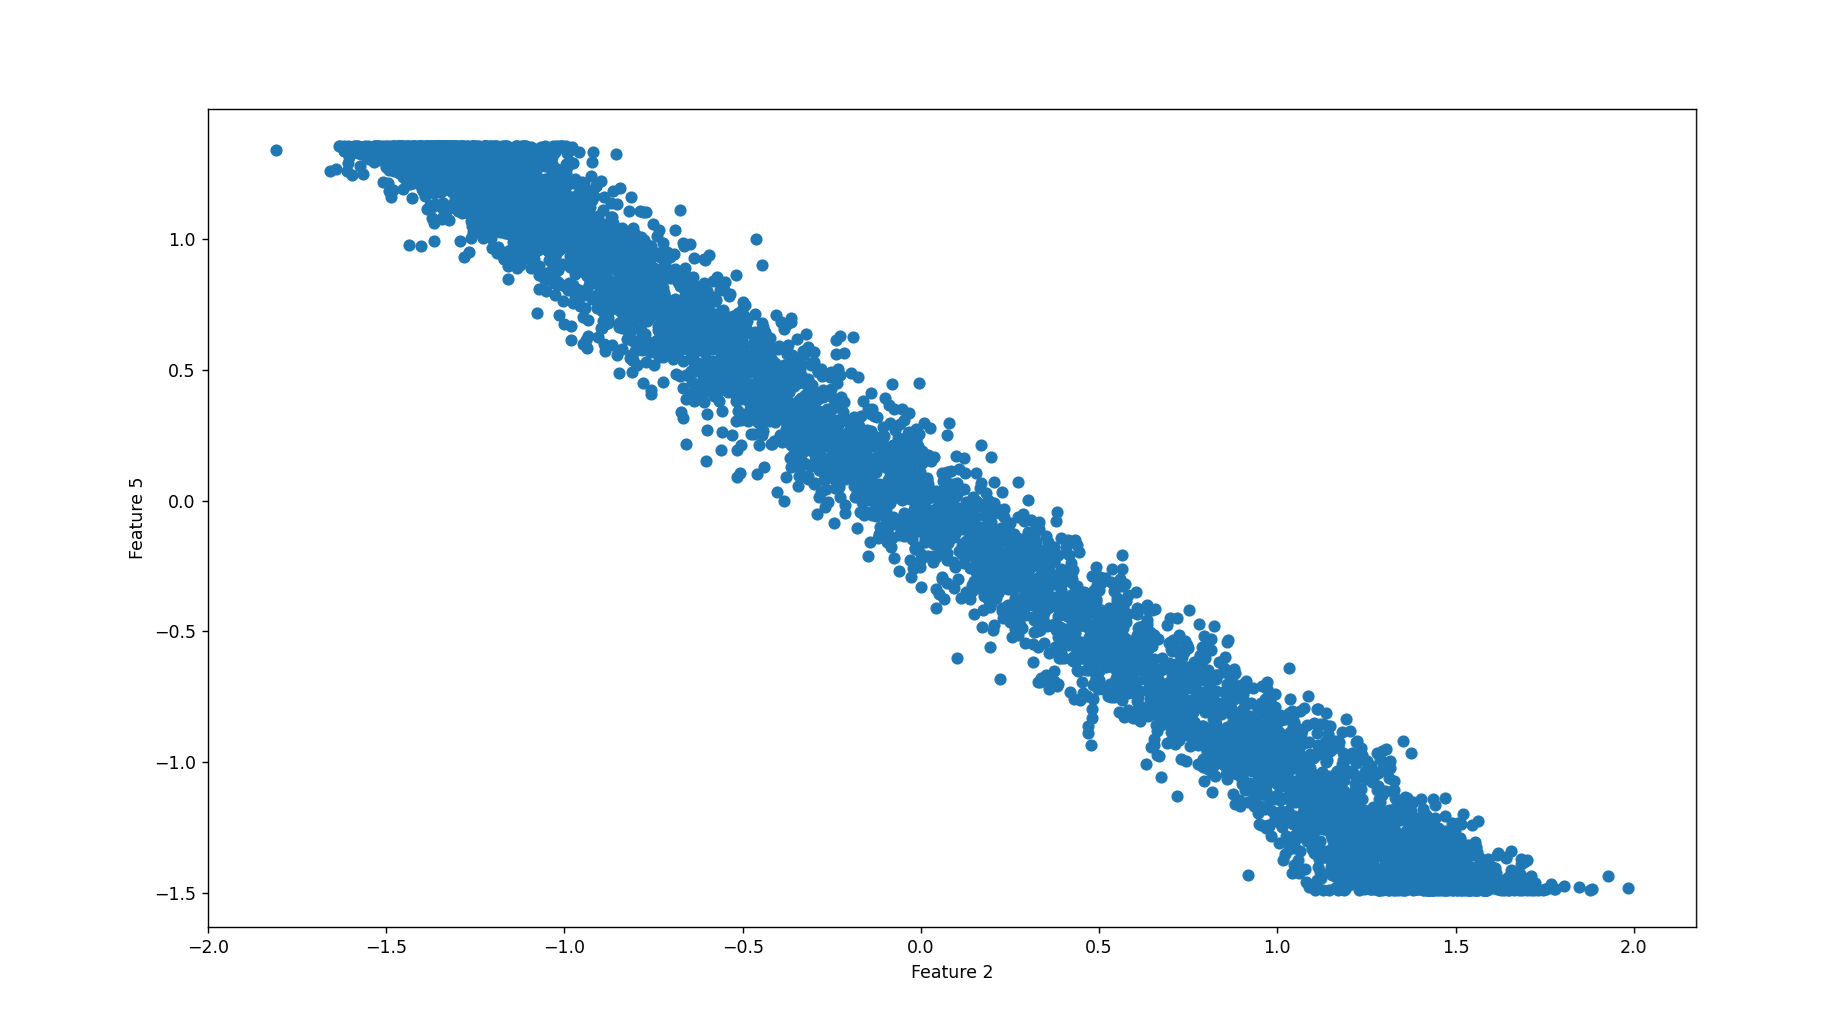
\includegraphics[width=\textwidth]{images/feature_2_5_correlation.png}
    \caption{Here there is a clear linear correlation between feature \textit{x2} and \textit{x5}, but very noisy}
    \label{fig:corr25}
\end{figure}

\begin{figure}[h]
    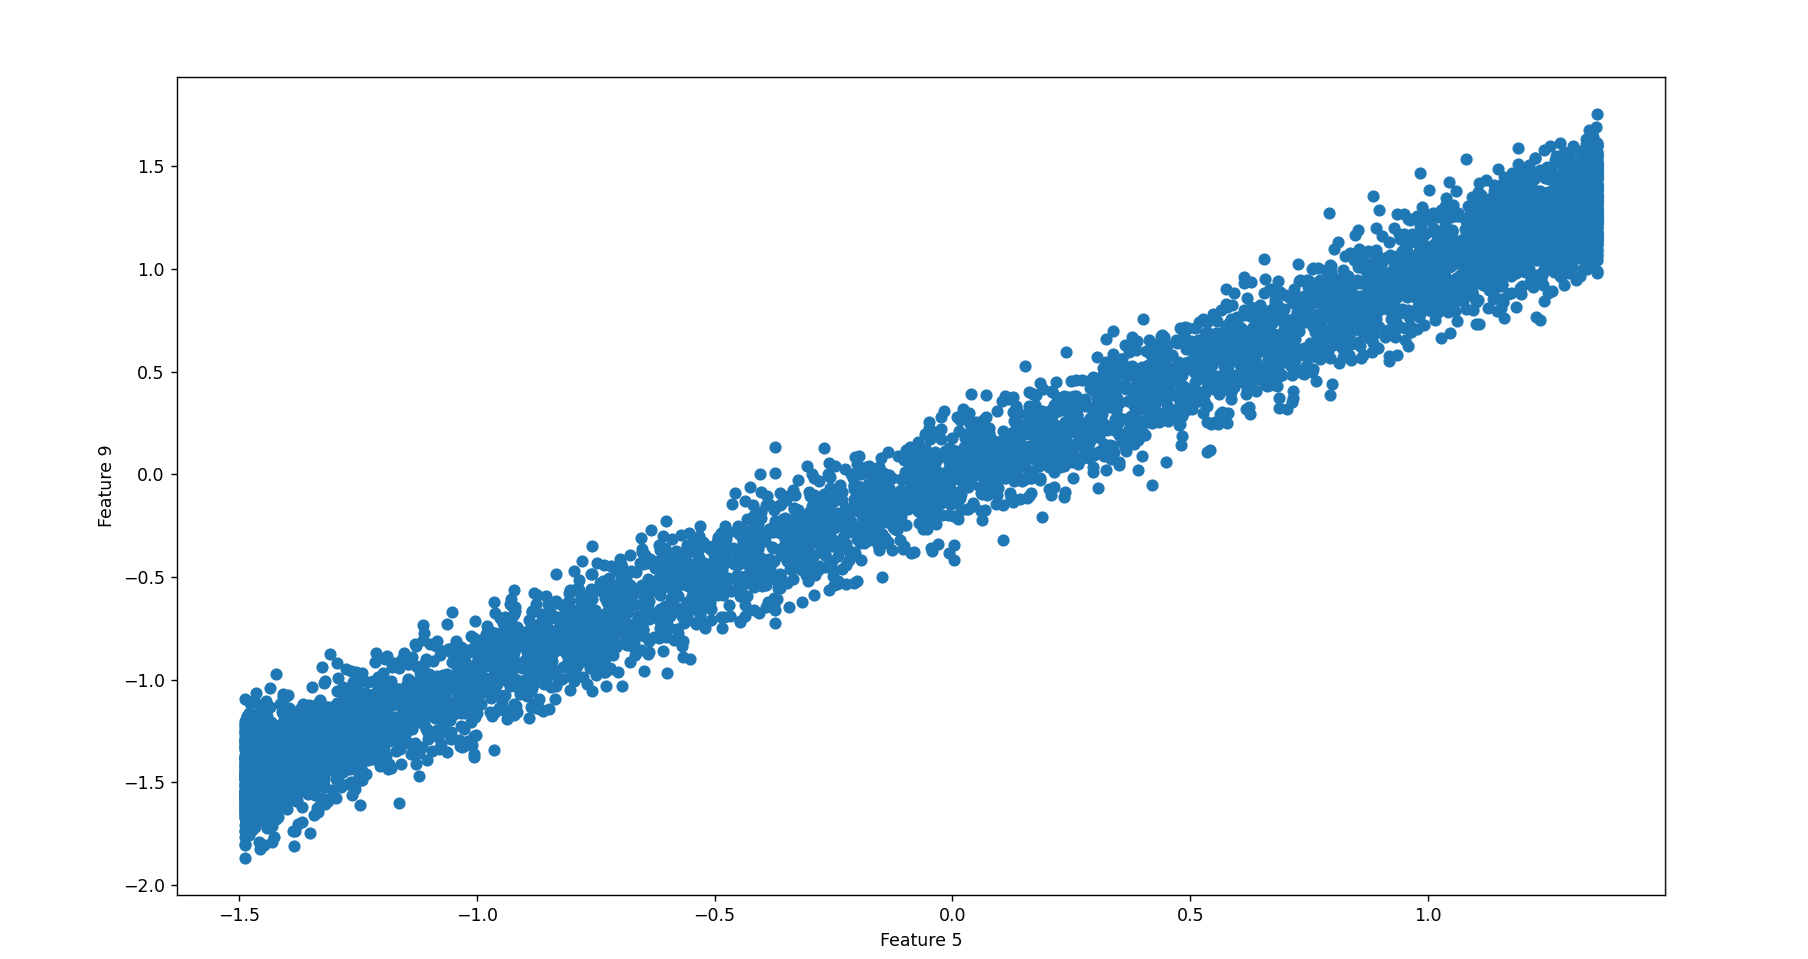
\includegraphics[width=\textwidth]{images/feature_5_9_correlation.png}
    \caption{Another correlation is also present between feature \textit{x5} and \textit{x9} (with a negative coefficent)}
    \label{fig:corr59}
\end{figure}

One possibility in this case during the preprocessing of the data is to remove the correlated features and leave only one of them to avoid redundancy of the data.\\
I don't follow this approach because there is a sensibile noise in the correlation and removing some features can lead to also removing this noise that can encode important information for the model.\\


\subsection{Feature expansion}
To being able to express non-homogeneous linear separators (hyperplane that don't pass through the origin) I add a constant feature of value $1$ to each point in the dataset.\\
Let $\bf(x)$ be any point in the dataset and $\bf(w)$ be the linear separator, if we define $x' = ({\bf x}, 1)$ we can define $w' = ({\bf} w, c)$, in that way: $${w'}^T x' = ({\bf w}^T {\bf x} + c)$$\\

\newpage
\section{Perceptron}

The first algorithm that I implemented is the perceptron algorithm.\\
The perceptron algorithm is used to learn linear classifiers.\\
linear classifiers are identified by an hyperplane that separe the input space into two halfspaces, one positive and one negative.\\
The positive halfspace is called so because the dot product with the normal vector that identify the hyperplane and any point in that space is positive, similary the negative halfspace has always negative dot products.\\
One important property of the Perceptron is the convergence (to the ERM) in a finite number of step if the dataset is lineary separable.\\
This properties is stated by the \textbf{Perceptron Convergence Theorem}:

\textit{Let $(\boldsymbol{x}_1 , y_1 ), \dots, (\boldsymbol{x}_m , y_m)$ be a linearly separable training set. Then the Perceptron algorithm returns a linear classifier with zero training error in a finite number of updates}
$$
M \leq \left(\underset{\boldsymbol{u} : \gamma(\boldsymbol{u}) \geq 1}{\min} \Vert \boldsymbol{u} \Vert^2 \right) \ \left( \underset{t = 1, \dots, m}{\max} \Vert \boldsymbol{x}_t \Vert^2 \right)
$$

where $\gamma (\boldsymbol{u})$ is the margin obtained by the linear separator $\boldsymbol{u}$\\ 
 
Is possible to show also a bound for non lineary separable cases:\\

$$
M \leq \sum_{t=1}^{T} h_{t}(\boldsymbol{u}) + (\Vert \boldsymbol{u} \Vert X)^2 + \Vert \boldsymbol{u} \Vert X \sqrt{\sum_{t=1}^{T}h_t (\boldsymbol{u})} \quad \text{for all}\ \boldsymbol{u} \in \mathbb{R}^d    
$$

This shows a bound on the number of mistakes made by the Perceptron algorithm on any data sequence of arbitrary length $T$.\\
$h_{t}(\boldsymbol{u})$ is the hinge loss for the $t$-example.\\

\subsection{Naive version}
\begin{algorithm}[H]
    \SetAlgoLined
    \DontPrintSemicolon
    \caption{The Perceptron algorithm}
    \KwIn{Training set $(\boldsymbol{x}_1 , y_1 ), \dots, (\boldsymbol{x}_m , y_m)$}
    $\boldsymbol{w} = (0, \dots, 0)$\\
\While{true} {  
    \For(\tcp*[f]{(epoch)}){$i = 1, \dots, m$}{
        \uIf{$y_i \boldsymbol{w}^{\top}\boldsymbol{x}_i \leq 0$}{
            $\boldsymbol{w} \leftarrow \boldsymbol{w} + y_i \boldsymbol{x}_i$ \tcp*[f]{(update)}\\ 
        }    
    }
    \uIf{no update in last epoch} {
        \textbf{break}
    } 
   }
   \KwOut{$\boldsymbol{w}$}
\end{algorithm}

My implementation slightly varies from the presented pseudocode:
While the above on keep running until convergence if the training set is not lineary separable (as in this case) we never converge and so the algorithm never terminates.\\
To avoid this I use an additional parameter 'max\_epoch' that limits the number of epoch which tha algorithm can run.\\
I choose to use a fixed value of 20 for this parameter both for the naive case and over the feature expanded dataset presented in the next section.\\
Training the perceptron algorithm with the preprocessing methodology described in the previous chapter (For all the algorihtms I describe I trained it with the default command line options), I have obtained a training error of $0.322625$ and a test error of $0.326$.\\
The linear separator founded by the perceptron algorihtm has the following features:\\\\
(0.55604295,  1.97486085, -2.58700382, -1.74490783,  1.91766823, -3.89876104,\\
 -0.02419966,  3.06371997,  0.21648717, -0.79054099,  1)
(Recall the features are 11 because we add a constant feature of 1 to the dataset to being able to express non-homogeneous linear hyperplane).\\

\subsection{Feature Expansion of 2nd degree}

I also trained the perceptron algorihtm on a second degree polynomial feature expanded dataset.\\
In this version of the algorithm is possible to express hyperplane in a high dimensional feature space, and this can also be interpreted as a polynomial curve (of second degree in this case) in the original space.\\
For this reason the training and test error of the resulting predictor are significantly better than the previous version.\\
Specifically I obtained a training error of 0.085375, and a test error of 0.087.\\
This are the features obtained:\\\\
(1.87559817e+01  1.13401244e+00  7.68047788e+00 -1.32276315e+01\\
  1.73791816e+01 -5.35283741e+00  1.04738036e+01  6.65533633e+01\\
  3.38354273e+01  5.20890557e+00 -1.40000000e+01 -2.37767269e+00\\
 -1.15700558e+01  3.58887386e+00 -7.70998879e+00 -3.37225323e+00\\
  8.62691037e+00  5.29455094e+00  7.16899813e+01 -2.75843723e+00\\
 -1.44740075e+01  1.87559817e+01  1.58098829e+00 -2.16046998e+01\\
  4.71738784e+00 -9.24568568e-01  2.31787163e+00 -6.88714236e-01\\
  6.36558311e+00  2.24640419e+02 -3.01817078e+01  1.13401244e+00\\
 -1.01581267e+01 -5.54650087e+00 -1.37119017e+01  5.92267047e+00\\
  6.13176127e+00 -1.91940656e+01  1.20197686e+01 -3.78679497e+00\\
  7.68047788e+00 -4.32369339e+00 -2.30745221e-01 -8.05450142e+00\\
  1.43389046e+00 -7.36485907e+01  4.14731220e+00  9.17178493e-01\\
 -1.32276315e+01  9.31783828e-01 -2.90129736e+01  1.10054038e+01\\
  9.29221437e+00  5.16458889e-02  5.24165775e+00  1.73791816e+01\\
 -3.39061351e+00  1.79056771e+01  1.68705706e+01  1.02044524e+01\\
 -7.88104212e+00 -5.35283741e+00  4.04206126e+00  1.28786306e+01\\
  1.01040343e+01  9.69582051e+00  1.04738036e+01  1.03988287e+01\\
  2.78928092e+00 -2.37491314e+01  6.65533633e+01  8.51087821e-01\\
  6.32907160e+00  3.38354273e+01 -2.72097857e+00  5.20890557e+00\\
 -1.40000000e+01) \\
\newpage
\section{Support Vector Machine}
% short description of the algorithm
The Support Vector Machine (SVM) algorithm learn linear classifiers, finding a linear classifier that is the \textbf{maximum margin separator hyperplane} and so achive the maximum margin from all the point in the training set.\\

Given a linearly separable training set $S = \{(\boldsymbol{x}_1, y_1), \dots, (\boldsymbol{x}_n, y_n)\} \in \mathbb{R}^d \times \{-1, 1\}$ it's possible to find this hyperplane solving the following convex optimization problem with linear constraints.\\ 
\begin{align*} 
    & \underset{\boldsymbol{w} \in \mathbb{R}^d}{\min} \ \frac{1}{2} \Vert \boldsymbol{w} \Vert^2 \\
    & \text{s.t.} \ y_t \boldsymbol{w}^\top \boldsymbol{x}_t \geq 1 \ \text{for} \ t = 1, \dots, m 
\end{align*}\\


In case the training data is not separable, we try to minimise both how much of each constraint is violated and the margin of the separator.\\
We express this as another convex problem using the slack variables $\xi_t$ and a regularisation coefficient $\lambda$.
If the regularisation coefficient is large, the algorithms will generate a predictor that allows more classification error in the training set.\\
Conversely, if $\lambda$ is small, we try to minimise the classification error we have made.\\
Usually for $\lambda$ too small, we try to minimise the misclassification, so the training error is small and we are likely to overfit.\\
Instead, for choices of $\lambda$ too large, we have a high training error, and if the test error is also high, we will underfit. \\
In the next subsection \ref{sub:hyptun}, I describe how I choose the hyperparameter of the regularisation coefficient and how the test and training errors vary when I change it more precisely.\\ 

\begin{align*}
    \underset{(\boldsymbol{w}, \boldsymbol{\xi}) \in \mathbb{R}^{d+m}}{\min} \quad & \frac{\lambda}{2} \Vert \boldsymbol{w} \Vert^2 + \frac{1}{m} \sum_{t = 1}^m \xi_t \\
    \text{s.t.} \quad & y_t \boldsymbol{w}^\top \boldsymbol{x}_t \geq 1 - \xi_t & t = 1, \dots, m \\
    & \xi_t \geq 0 \ \text{for} & t = 1, \dots, m
\end{align*}

Now, fix $\boldsymbol{w} \in \mathbb{R}^d$, we can see $\xi_t = \left[1 - y_t \boldsymbol{w}^\top \boldsymbol{x}_t \right]_+$ which is the hinge loss  $h_{t}(\boldsymbol{w})$.\\

The SVM problem can be rewritten as $$\underset{\boldsymbol{w} \in \mathbb{R}^d}{\min} \ \frac{\lambda}{2} \Vert \boldsymbol{w} \Vert^2 + \frac{1}{m} \sum_{t = 1}^m h_{t}(\boldsymbol{w})$$.\\

The optimization problem that describe the Support Vector Machine is optimized using the Pegasos algorithm.\\
The Pegasos algorithm is a variant of the Stocastic Gradient Descent algorithm, where at each step a point (or a set of points in the mini-batch variant) is sampled randomly from the training set
and the current predictor is updated with the negative gradient of the loss of that training example weighted by a learning rate factor $\eta_t$.\\
In case of Pegasos the learning rate factor $\eta_t$ is choose at each step as $\frac{1}{\lambda t}$.\\
I implement the Pegasos algorithm using the standard variant with the \textit{hinge} loss, and with the \textit{logistic} loss (Described in the Logistic regression subsection \ref{sub:logreg}).\\
Both this functions are convex upper bounds of the zero-one loss, and the $\lambda$ regularization parameter allow to have a $\lambda$-strongly convex function to minimize with the gradient descent.\\
% TODO: refer to the OGD and Pegasos bound on function minimum this is why we say that the function to minimize are $\lambda$-strongly convex

\subsection{Naive}
As I previously said I implemented Pegasos using two surrogate losses: hinge loss and logistic loss.\\
Now I describe the implementation with hinge loss, that differs from the logistic one only by the update step.\\ 
Recall that the hinge loss is defined as $l(y, \hat{y}) = \max\{0, 1 - y_t \hat{y}\}$\\
Given $Z_t = (X_t, Y_t)$ a random sample from the training set, the update rule for Pegasos is:\\
$$\boldsymbol{w}_{t+1} = \boldsymbol{w}_t - \eta_t \nabla\ell_{Z_t}(w_t)$$

Let be $s_t$ the realization for the random variable $Z_t$\\ 
Where $\ell_{s_t}(w) = \left[1 - y_{s_t} \boldsymbol{w}^T x_{s_t}\right]_+ + \frac{\lambda}{2} ||w||^2$ so
$$\nabla\ell_{s_t}(w) = -y_{s_t} x_{s_t} \mathbb{I}\{h_{s_t}(\boldsymbol{w}) > 0\} + \lambda w $$
Let $\boldsymbol{v_t} = y_t x_t I\{h_t(\boldsymbol{w_t}) > 0\}$ and choosing $\eta_t = \frac{1}{\lambda t}$ we have
$$\boldsymbol{w}_{t+1} = \boldsymbol{w}_t (1 - \frac{1}{t}) + \frac{1}{\lambda t} \boldsymbol{v_t}$$

\subsubsection{Implementation details}
I adapted this version of the algorithm from \textit{Pegasos: Primal Estimated sub-GrAdient SOlver for SVM}\cite{Pegasos_paper}\\

\begin{algorithm}[H]
    \SetAlgoLined
    \DontPrintSemicolon
    \caption{Pegasos Algorithm}
    \KwIn{$S$, $\lambda$, $T$}
    \For{$t = 1, 2, \dots, T$}{
        Choose $i_t$ uniformly at random.\\
        Set $\eta_t = \frac{1}{\lambda t}$\\
        \If{$y_{it} \boldsymbol{w}_t^T x_{i_{t}} < 1$}{
            Set $\boldsymbol{w}_{t+1} \leftarrow (1 - \eta_t \lambda)\boldsymbol{w}_t + \eta_t y_{it} \boldsymbol{x}_{i_{t}}$
            }
            \Else {
                Set $\boldsymbol{w}_{t+1} \leftarrow (1 - \eta_t \lambda)\boldsymbol{w}_t$
        }
    }    
    Output $\boldsymbol{w}_{T+1}$
\end{algorithm}

The name of the variables are adapted to be consistent with the pseudo code reported.\\
Between the code presented in the lecture and this one presented in the paper there are some differences:\\
\begin{itemize}
    \item The gradient descent update is written in a slightly different way using a conditional statement instead of the classical indicator function, I choose to remain consistent also with this stilistic choice.\\
    \item Instead of return the average of all the weight vector calculated at each step, the paper returns only the last one.\\ 
    The authors indicate that they note an improvement in performance by returning the last vector instead of the average.\\ 
    I accept also this variation.\\
    \item The Pegasos pseudocode also describes an optional projection step to clamp the magnitude of the linear predictor, but I don't incorporate it.\\ 
\end{itemize}

% TODO: mini-batch: if I test also the mini-batch I should report if I notice some improvment and how the algorithm change based on the hyperparameter
Two other approaches that the author suggest but I don't experiment are:
\begin{itemize}
    \item The author also provides a \textbf{mini-batch} version of the Pegasos algorithm.\\ 
    The chosen batch is a set of $k$ random samples from the training set, and the linear predictor is updated with the average loss gradient of all incorrectly predicted samples in the batch.\\
    The batch size $k$ can be chosen in advance or treated as another hyperparameter.\\
    \item \textbf{sampling without replacement}: a random permutation of the training set is chosen and the updates are performed in order on the new sequence of data.
    In this way, a training point is sampled only once in an epoch.\
    After each epoch, we can choose whether to resume sampling the data sequentially according to the same permutation, or to create a new permutation and sample according to that new order.\\
    Although the authors report that this approach gives better results than uniform sampling as I did, I haven't experimented with this variant of the algorithm.\\    
\end{itemize} 

\subsubsection{Hyperparameter tuning} \label{sub:hyptun}
Unlike the perceptron, the Pegasos algorithm had a hyperparameter to choose from: The regularisation coefficient $\lambda$.\\
To choose the best hyperparameter for this algorithm (and the others that I will implement), I choose the grid search method.\
I divide the training set into 2 different subsets: $S_{traing}$ and $S_{dev}$.\\
The validation set ($S_{dev}$) is used as a surrogate test set to get an estimate of the risk.\\
I choose a finite subset of the possible hyperparameter values ($\Theta_0 \subseteq \Theta$) and for each of them I create a predictor $h_\theta$ which is trained with the chosen hyperparameter on $S_{train}$.\\
The risk is then estimated using the validation error on each predictor, and the one with the lower risk is chosen.\\
The implementation of the grid search in my codebase is in the function 'grid\_search', I used python know arguments to pass a dictionary where the key is the name of the hyperparameter (the same as used as an argument in the training algorithm) and the value is an iterator containing the subset of possible values ($\Theta_0$).\\ 
In this case, I choose the set $\Theta_0 = \{ 0.0001, 0.001, 0.01, 0.1, 1, 10, 100 \}$.\\

\begin{center}
    \begin{tabular}{| c | c | c |}
        \hline
        $\lambda$ & $S_{val}$ & $S_{train}$ \\
        \hline
        0.0001 & 0.3725 & 0.3521666 \\
        \hline
        0.001 & 0.2925 & 0.281333 \\
        \hline
        0.01 & 0.273 & 0.27 \\
        \hline
        \textbf{0.1} & \textbf{0.267} & \textbf{0.2661666} \\
        \hline
        1 & 0.273 & 0.269333 \\
        \hline
        10 & 0.279 & 0.2775 \\
        \hline
        100 & 0.2805 & 0.276333 \\
        \hline
    \end{tabular}
    \\
    The values $S_{val}$ and $S_{train}$ while $\lambda$ changes.\\
\end{center}

Looking at the table we can deduce for which choice of $\lambda$ we underfit and overfit and in our case the sweet spot is the value for $\lambda = 0.1$.\\
The test error for the best predictor is 0.2935.\\
We can also see that for smaller value of lambda we have an high test error and model is overfitting while for large value are likely to underfit.\\
The weight for the Pegasos algorithm are the following: \\
% TODO: file esterno per i pesi del linear predictor
0.2080856  -0.0066276   0.07067274 -0.26477777  0.24795273 -0.06704699\\
0.28821758  0.65130349  0.16619769 -0.06650096 -0.0724

\subsection{Logistic regression} \label{sub:logreg}
Logistic regression aim to learn the function $\eta(\boldsymbol{x}) = \mathbb{P}(Y = +1\ |\ \textbf{X} = \boldsymbol{x})$.\\
The implementation of logistic regression differs from the standard Pegasos because it uses the logistic loss as surrogate loss and not hinge.\\
The logistic loss is defines ad follows: $$\ell(y, \hat{y}) = \log_2 (1+e^{-y\hat{y}}).$$\\
So the gradient descent update becomes: $$\boldsymbol{w}_{t+1} = \boldsymbol{w}_t + \eta_t \sigma(-y_t \boldsymbol{w}^T \boldsymbol{x}_t) y_t \boldsymbol{x}_t$$\\
I choose the regularization parameter as described in the previous subsection and obtained the following results.\\
\begin{center}
    \begin{tabular}{| c | c | c |}
        \hline
        $\lambda$ & $S_{val}$ & $S_{train}$ \\
        \hline
        0.1 & 0.278 & 0.2718333 \\
        \hline
        \textbf{1} & \textbf{0.2735} & \textbf{0.274333} \\
        \hline
        10 & 0.28325 & 0.27816 \\
        \hline
        100 & 0.2805 & 0.278166 \\
        \hline
    \end{tabular}
    \\
    The values $S_{val}$ and $S_{train}$ while $\lambda$ changes for the logistic loss.\\
\end{center}

I have choosen the hyperparameter $\lambda = 1$ and obtained a test error of: 0.292.\\

\subsection{Feature Expansion}
I have also trained the two previous algorithms over the polynomial feature expansion of second degree of the whole dataset.\\
Like in the case of perceptron, since we are able to express a separator in an high dimension we obtain better results than the naive version (at the cost of an increasing number of features in the dataset).\\  
\subsubsection{Pegasos}
This are the following validation and development errors training the Pegasos algorithm the same set of values choosen for the hyperparameter $\lambda$ as in the naive version.\\

\begin{center}
    \begin{tabular}{| c | c | c |}
        \hline
        $\lambda$ & $S_{val}$ & $S_{train}$ \\
        \hline
        \textbf{0.001} & \textbf{0.045} & \textbf{0.039833} \\
        \hline
        0.01 & 0.06 & 0.050166 \\
        \hline
        0.1 & 0.0955 & 0.08833 \\
        \hline
        1 & 0.1725 & 0.1525 \\
        \hline
        10 & 0.219 & 0.211 \\
        \hline
        100 & 0.256 & 0.246 \\
        \hline
        1000 & 0.2635 & 0.25233 \\
        \hline
    \end{tabular}
\end{center}

The test error obtained training the predictor on the whole training set with the regularization coefficent of $0.001$ is $0.053$ with a training error of $0.044125$.\\

\subsubsection{Logistic Regression}

\begin{center}
    \begin{tabular}{| c | c | c |}
        \hline
        $\lambda$ & $S_{val}$ & $S_{train}$ \\
        \hline
        \textbf{0.1} & \textbf{0.11} & \textbf{0.1035} \\
        \hline
        1 & 0.1675 & 0.15 \\
        \hline
        10 & 0.197 & 0.188 \\
        \hline
        100 & 0.2595 & 0.2485 \\
        \hline
        1000 & 0.2505 & 0.2385 \\
        \hline
    \end{tabular}
\end{center}

The test error obtained for the feature expanded logistic regression (with $\lambda = 0.001$) is $0.1125$ with a training error of $0.1055$.\\
Note that for both versions of logistic regression, not all of the $\lambda$ parameters used for the hinge loss SVM in the grid search are used in this case.\\ 
This is because for values that are too small, I get an overflow error when exponentiating in the sigmoid function.\\ 
These values, for which the gradient update calculation is not feasible, are simply discarded.\\

\newpage
\section{Kernel}
In the previous section I have showed the benefit of training the algorithm in an high-dimensional space.\\
This came with the cost of increasing sensibily the number of the feature even in case of a simple polynomial feature expansion of degree 2.\\
We can have the performance improvement obtained with feature expansion without increasing the dimensionality of the dataset using the kernel trick.\\
Instead of computing the feature expansion map on evry point and then computing the dot product with the expanded linear predictor we can use a kernel $K$ that calculate the dot product of two expanded vector without explicitly calculate the expansion.\\
Let the feature expansion be $\phi(x)$ a kernel $K$ for the feature expansion is defined as $$K(x, x') = \phi(\boldsymbol{x})^T \phi(\boldsymbol{x'})  for all \boldsymbol{x}, \boldsymbol{x'} \in R$$\\
The two kind of kernel used in the project are the \textbf{Polynomial kernel} and the \textbf{Gaussian kernel}.\\
The polynomial kernel of degree $n$ is defined as $$K_n(x, x') = (1 + \boldsymbol{x}^T \boldsymbol{x'})^n$$
The gaussian kernel of parameter $\gamma$ is defined as $$K_\gamma(x, x') = exp(-\frac{1}{2\gamma}||\boldsymbol{x} - \boldsymbol{x'}||^2)$$
Note that both the kernels accept a parameter (a degree in the polynomial case and gamma for gaussian one) this becomes another hyperparameter of the learning algorithm
and it's choosen with the same hyperparameter tuning procedure descripted in the previous chapters.\\ 
Each kernel induce a linear space defined as a set of linear combination of functions $K(\boldsymbol{x}, \dot)$.\\
\begin{align*}
    \mathcal{H}_K \equiv \left\{ \sum_{i=1}^N \alpha_i K(\boldsymbol{x}_i, \cdot) : \boldsymbol{x}_1, \dots, \boldsymbol{x}_N \in \mathcal{X}, \alpha_1, \dots, \alpha_N \in \mathbb{R}, N \in \mathbb{N} \right\}
\end{align*}
This spaces are called Reproducible Kernel Hilbert Space (RHKS).\\
A linear predictor trained in these linear spaces induced by kernels can overfit; in the case of polynomial kernels, we can choose a degree that is too high and obtain a curve with more degrees of freedom, which is more likely to separate the training data and obtain a small training error.\\
For the Gaussian, we should know that the parameter $\gamma$ is the width of the Gaussian centre at the training point.\\
This means that if $\gamma$ is too small, we are likely to have a small training error (we only look at the labels of the nearest points) and overfit.\\


\subsection{Implementation details}
I used two classes with the '\_\_call\_\_' python magic method to implement the kernels functions.\\
Both takes two parameter $X$ and $X2$.\\
They can take two vectors and the kernel behave as mathematicly defined or the parameter can be 2 matrices of size $m$ x $d$ and $n$ x $d$.\\
In the second case a new matrix $\boldsymbol{K}$ ($m$ x $n$) defined as $\boldsymbol{K}_{i, j} = K(X_i, X2_j)$.\\
This is particular useful to avoid python for loops and delegate the computations to the optimize implementation of the numpy primitives.\\

\begin{python}
def __call__(self, X: np.ndarray, X2: np.ndarray):
    if X2.ndim == 1:
        return np.power(np.dot(X, X2) + 1, self.degree)
    elif X2.ndim == 2:
        return np.power(np.dot(X, X2.T) + 1, self.degree)
\end{python}
Implementation of the polynomial kernel over $X$ and $X2$.\\

\begin{python}
    def __call__(self, X: np.ndarray, X2: np.ndarray):
        if X2.ndim == 1:
            dist = np.linalg.norm(X - X2, 2, axis=1)
        elif X2.ndim == 2:
            dist = np.linalg.norm(X[:, np.newaxis, :] - X2[np.newaxis, :, :], axis=2)
        return np.exp(-dist / self.gamma)
\end{python}
Implementation of the gaussian kernel over $X$ and $X2$ with the parameter gamma $\gamma$ .\\
% add the two implementations with code

\subsection{Kernelized Perceptron}

The first algorithm I implement using the kernel trick is the perceptron.\\
following I provide a pseudocode taken from the lecture notes about this algorihtm.\\ 

% pseudocode

\begin{algorithm}[H]
    \SetAlgoLined
    \DontPrintSemicolon
    \caption{Kernel Perceptron}
    $S \leftarrow \emptyset$ \\
    \For{$t = 1, 2, \dots$}{
        Get next example $(\boldsymbol{x}_t, y_t)$ \\
        Compute $\hat{y_t} = \text{sgn}\left(\sum_{s \in S}\ y_s K(\boldsymbol{x}_s, \boldsymbol{x}_t) \right)$ \\
        \If{$\hat{y_t} \neq y_t$}{
            $S \leftarrow S \cup \{t\}$
        }
    }
\end{algorithm}

% Difference between implementation and pseudocode
Looking at the implementation, I have implemented the kernel perceptron algorithm with an array $\alpha$ of integer weights for each point of the training set instead of using a set $S$, this may seem different from the pseudocode presented, but we can interpret $\alpha$ as representing a multi-set and have an equivalent algorithm.\\
This choice, taken from the pseudo code of the kernelized perceptron in the Pegasos paper, is adopted because we can express the summation more simply and efficiently thanks to the numpy primitive such as 'np.dot'.\\

% Hyperparameter
With the kernel version we have a new hyperparameter: The type of kernel used with its parameter (the degree for polynomials and the $\gamma$ for Gaussians).\\
We choose the best hyperparameter, as described in the previous chapters.\\
Among the possible values, we choose 1, 2, 3, 4 for the possible degrees of the polynomial kernel, and 0.01, 0.1, 1 and 10 for the possible values of $\gamma$.\\

% results
\begin{table}[]
    \begin{tabular}{|c|c|c|c|}
        \hline
        Polynomial Kernel n & Gaussian Kernel $\gamma$ & $S_{val}$ & $S_{train}$ \\ \hline
        1 & & 0.339 & 0.3251666 \\ \hline
    2 & & 0.0685 & 0.06633 \\ \hline
    \textbf{3} & & \textbf{0.0585} & \textbf{0.048} \\ \hline
    4 & & 0.06 & 0.031666 \\ \hline
    & 0.01 & 0.2075 & 0.0 \\ \hline
    & 0.1 & 0.1805 & 0.0 \\ \hline
    & 1  & 0.0685 & 0.0015 \\ \hline
     & 10 & 0.072 & 0.01366 \\ \hline    
    \end{tabular}
    \label{tab:kper}
\end{table}
We can make some considerations about the data in the table \ref{tab:kper} based on the previous theoretical section of this chapter:
% TODO: better rewrite
We can see that when using the Gaussian kernel, we have a training error $S_{train} = 0$ for the smaller value of $\gamma$, 
This can be explained by observing that if the radius of the Gaussians is too small, the Gaussians over the training points do not interact and for each training point the algorithm behaves as a K-NN with $K = 1$ and for the same reason the training error is 0.\\
It's also possible to know in which cases for the polynomial kernel we overfit, observe that in the case of $n = 4$ we have a value $S_{val}$ significantly greater than $S_{train}$.\\
In contrast, for $n < 3$ we also have both an high $S_{val}$ and an high $S_{train}$, indicating underfitting.\\
\subsection{Kernelized Pegasos}

\begin{algorithm}[H]
    \SetAlgoLined
    \DontPrintSemicolon
    \caption{Pegasos Algorithm}
    I implement the kernelized version of the Pegasos algorithm following the pseudocode from the paper, reported here:
    \KwIn{$S$, $\lambda$, $T$}
    Initialize: Set $\boldsymbol{\alpha}_1 = 0$\\
    \For{$t = 1, 2, \dots, T$}{
        Choose $i_t \in {0, \dots, |S|}$ uniformly at random.\\
        
        For all $j \neq i_t$, set $\boldsymbol{\alpha}_{t+1}[j] = \boldsymbol{\alpha}_t[j] $\\
        \If{$y_{i_{t}} \frac{1}{\lambda t} \sum_{j}{\boldsymbol{\alpha}_t[j] y_{i_t} K(\boldsymbol{x}_{i_t}, x_j)} < 1$}{
            Set $\boldsymbol{\alpha}_{t+1}[i_t] = \boldsymbol{\alpha}_t[i_t] + 1$
        } 
        \Else {
            Set $\boldsymbol{\alpha}_{t+1}[i_t] = \boldsymbol{\alpha}_t[i_t]$
        }

    }
    Output $\boldsymbol{\alpha}_{T+1}$\\
\end{algorithm}

% results
As in the previous algorithm, I fixed a number of rounds $T = 100000$ and tuned the algorithm over the hyperparameters $\lambda$ (the regularization coefficient) and a kernel that can be either polynomial of degree $1,2,3$ or $4$, or gaussian with a $\gamma$ parameter of one between ${0.01, 0.1, 1, 10}$.\\
\begin{table}[]
    \begin{tabular}{|l|l|l|l|l|}
    \hline
    $\lambda$ & Polynomial Kernel n & Gaussian Kernel $\gamma$ & $S_{val}$ & $S_{train}$ \\ \hline
    0.001 & 1 &  & 0.275 & 0.2738333333333333 \\ \hline
    0.001 & 2 &  & 0.0605 & 0.055 \\ \hline
    0.001 & 3 &  & 0.053 & 0.045 \\ \hline
    0.001 & 4 &  & 0.057 & 0.026166666666666668 \\ \hline
    0.001 & & 0.01 & 0.1675 & 0.0 \\ \hline
    0.001 & & 0.1 & 0.1465 & 0.0 \\ \hline
    0.001 & & 1 & 0.114 & 0.06633333333333333 \\ \hline
    0.001 & & 10 & 0.157 & 0.13683333333333333 \\ \hline
    0.01 & 1 &  & 0.2755 & 0.26916666666666667 \\ \hline
    0.01 & 2 &  & 0.055 & 0.04833333333333333 \\ \hline
    0.01 & 3 &  & 0.049 & 0.03716666666666667 \\ \hline
    0.01 & 4 &  & 0.051 & 0.025 \\ \hline
    0.01 & & 0.01 & 0.167 & 0.0 \\ \hline
    0.01 & & 0.1 & 0.15 & 0.0 \\ \hline
    0.01 & & 1 & 0.2275 & 0.21266666666666667 \\ \hline
    0.01 & & 10 & 0.2495 & 0.246 \\ \hline
    0.1 & 1 &  & 0.2645 & 0.26316666666666666 \\ \hline
    0.1 & 2 &  & 0.084 & 0.07616666666666666 \\ \hline
    \textbf{0.1} & \textbf{3} &  & \textbf{0.044} & \textbf{0.043} \\ \hline
    0.1 & 4 &  & 0.05 & 0.023166666666666665 \\ \hline
    0.1 & & 0.01 & 0.166 & 0.0 \\ \hline
    0.1 & & 0.1 & 0.1465 & 0.0 \\ \hline
    0.1 & & 1 & 0.2385 & 0.2255 \\ \hline
    0.1 & & 10 & 0.2545 & 0.257 \\ \hline
    1 & 1 & & 0.2725 & 0.2668333333333333 \\ \hline
    1 & 2 & & 0.144 & 0.131 \\ \hline
    1 & 3 & & 0.0825 & 0.072 \\ \hline
    1 & 4 & & 0.0535 & 0.029 \\ \hline
    1 & & 0.01 & 0.167 & 0.0 \\ \hline
    1 & & 0.1 & 0.1445 & 0.0 \\ \hline
    1 & & 1 & 0.2415 & 0.2245 \\ \hline
    1 & & 10 & 0.26 & 0.25883333333333336 \\ \hline
    10 & 1 & & 0.285 & 0.2796666666666667 \\ \hline
    10 & 2 & & 0.193 & 0.17766666666666667 \\ \hline
    10 & 3 & & 0.143 & 0.13383333333333333 \\ \hline
    10 & 4 & & 0.0705 & 0.05433333333333333 \\ \hline
    10 & & 0.01 & 0.1675 & 0.0 \\ \hline
    10 & & 0.1 & 0.1445 & 0.0 \\ \hline
    10 & & 1 & 0.2365 & 0.225 \\ \hline
    10 & & 10 & 0.274 & 0.265 \\ \hline
    100 & 1 & & 0.2805 & 0.27616666666666667 \\ \hline
    100 & 2 & & 0.2015 & 0.19333333333333333 \\ \hline
    100 & 3 & & 0.2185 & 0.21433333333333332 \\ \hline
    100 & 4 & & 0.111 & 0.10033333333333333 \\ \hline
    100 & & 0.01 & 0.169 & 0.0 \\ \hline
    100 & & 0.1 & 0.144 & 0.0 \\ \hline
    100 & & 1 & 0.2405 & 0.223 \\ \hline
    100 & & 10 & 0.2845 & 0.2813333333333333 \\ \hline
\end{tabular}
\label{tab:kpeg}
\end{table}

% 
The best hyperparameters obtained by the grid search procedure are a regularization coefficient $\lambda = 0.1$ and a polynomial kernel of degree 3.\\
We obtain a training error on the whole data set of 0.035875 and a test error of 0.043.\\
We can see from the test error that this is the best performing method implemented.\\
This is also because we are using a 3rd degree polynomial kernel and we are training a linear predictor in a higher dimensional space than the one I obtained with the 2nd degree polynomial expansion.\\
In the table \ref{tab:kpeg} we can also see for which values of $\lambda$ and kernel degree the predictor overfits, fixing the other hyperparameter.\\
Fixing the regularization coefficient $\lambda = 0.1$ we can experimentally confirm that for high degrees of the kernel (4) the predictor overfits and has a high validation error and for smaller values (1 or 2) it underfits.\\
Conversely, by fixing the chosen kernel and varying $\lambda$, we can see that $S_{val}$ is slightly higher for values of the regularization coefficient $< 0.1$ and we are probably overfitting, while for higher values the validation error is much higher and this can signal underfitting.\\

% introduction
%   - project description and technologies involved
% dataset analysis and preprocessing
%   - dataset description
%   - normalization (advantage from the theorical prospective) (avoid data leakage)
%   - standardization (advantage from the theorical prospective) (avoid data leakage)
%   - outliers removal
%   - feature correlation
%   - feature expansion
%     to being able to express non-homogeneous linear separator (separator that are not in the origin) we add a constant feature of one to the training set in this way... (formula) 
% Perceptron
%   - naive
%     - results
%   - with Feature expansion (degree 2)
%     - results
% Support Vector Machine (Pegasos)
%   - naive
%       - Hyperparameter tuning
%          grid search with his implementation
%       - implementation details
%           (compare the implementation with the one on the paper)
%           typo: the index i_t in the summation
%       - results
%           - Overfitting and under fitting (theoric view)
%   - logistic regression
%       - results
%           - Overfitting and under fitting (theoric view)
%   - with Feature expansion
%   - logistic regression with Feature expansion
% Kernels


% Bibliography
\begin{thebibliography}{unsrt}

    \bibitem{Pegasos_paper}
    Shai Shalev-Shwartz, Yoram Singer, Nathan Srebro, Andrew Cotter \emph{Pegasos: Primal Estimated sub-GrAdient SOlver for SVM}. https://home.ttic.edu/~nati/Publications/PegasosMPB.pdf
    
\end{thebibliography}

\end{document}